\doublespacing
\chap{Related Work} 
\label{chap:RelatedWork}

Image generation is a very diverse and constantly evolving area of computer vision. In the last few of years, generative neural networks have shown very promising results. In this chapter, we examine various generative model ranging from Boltzmann machines to the latest convolutional neural network based on generative models.
\section{Early Work}

There has been a lot of research going on in the area of generative models. One of the most proven models belongs to Restricted Boltzmann machine and Deep Belief Net [cite].

A Boltzmann machine is an approach for estimating the probability distribution function over binary vectors. Boltzmann machines which is  a energy based model were one of the first neural network models which showed that they can learn internal representations of the data \cite{Boltzman-Wiki}.
In this work they use Boltzmann machine to generate MNIST digits. The author uses persistent Markov chains for estimating model expectations. In this work, the author uses stochasti\label{chap:foo}c parameter approximation procedure with continuously decreasing learning rate. Also to estimate the data-dependent expectations, the author uses variational learning which in turn helped improve faster convergence. 

\par 

Deep Belief Network


\section{GAN Extensions}
In the work of coupled GAN \cite{Co-GAN}, the author used two pairs of generators and discriminators. This works targets learning of multi-domain images. The main contribution of this work lies in learning of a joint distribution of images covering two different domains. In this work, to restrict the image generated by two generators to share higher semantics, the author constrains the two generator to share weights at the first layer. The generator decodes information from higher to lower semantics where as discriminator which is a standard Convolutional Neural Network decodes the images in lower to higher semantics. Hence, the two discriminator last layer weights are also shared. The major issue with coupled adversarial network is training, since we have to tackle a lot of issues in training a single GAN.
\par

In the work of Stack GAN (SGAN)\cite{stacked-gan}, the author proposes top-down stack of GANs. Each generator takes higher representation and adds lower representation to it. Here authors for training  a adversarial network uses adversarial, entropy and conditional losses. By using entropy loss author tackles the issue of conditional model collapse. Conditional model collapse  is a  scenario	observed	when	the	GAN	starts	ignoring the noise variable(z). In this work to process all the variations for a image author uses multiple noise variable(z) in SGAN. The proposed model uses a bottom up discriminator as a encoder which at each level guides the generator in producing intermediary representation of an image.

In the work of LRGAN \cite{LR-GAN}, the author takes advantage of viewing image as layers. In this work author uses 2 kind of generators , one responsible for generating background and the other generating foreground. In this whole process background is generated ones but foreground is generated recursively with help of long term short memory neural network\cite{hochreiter1997long}.The purpose of long term short memory network is to  provides information to the foreground generator about what has been generated. Each time a foreground image is generated, it is copy and pasted on the previously stitched image after doing affine and spatial transformation\cite{1506.02025}. 



In the work of Information GAN, the author introduces new variable apart from noise in GAN framework. This term encourages high mutual information between generated samples and a small subset of latent variables. By this author forces high information content interesting aspects of the representation into the conditional variable. This work looked promising but when we tried to replicate the work, this model failed in producing consistent results with complex dataset.


\section{Improving GAN}

In the work of ADAGAN, author address the issue of model collapse. Model collapse happens when you have very diverse data-set and your GAN is not able to learn the whole distribution and end up learning some part of it. So the author proposes using GAN in boosting algorithm. This work shows promises of tackling the issue of highly diverse data-set by using bunch of weak GANs.
\par

In this work of Unrolled GAN, the author proposes solution for various issues in training GANs. 
In this work author uses unrolled optimization of discriminator objective function.  The optimal solution for a adverarial network will is $\theta^{*} =\left\{\theta^{*}_{G}, \theta^{*}_{D}\right\}$ has iterative solution using one of the optimization techniques such as SDG, Adam. Now, the author unrolls the discriminator K time to create a surrogate objective function for generator as shown in below equation 2.1. As we can see if K=0 the we have a standard GAN.
\begin{equation}
        \begin{aligned}
f_{k}{ \left( \theta _{g}, \theta _{d} \right) }=f \left( \theta _{g}, \theta _{d}^{K}{ \left( \theta _{g}, \theta _{d} \right) } \right)
\end{aligned}
\end{equation}

In this work \cite{1612.04021}, author proposes parallelization approach for tackling over-fitting and long training time problem with GAN. To explain over-fitting author uses analogy of a fighter and his trainer. In this, when a fighter is trained with a particular style of the trainer then in any fight the fighter will perform better when the style of opponent matches the trainer. Similarly if  we have a distribution with multiple modes and if discriminator is not able figure out the correct label then generator won't be motivated to over different modes. To tackle this problem, author uses multiple generator and discriminator where each pair of generator and discriminator share parameter which very unlike many another technique uses. Here to maintain same synergy across various pair, the discriminators are swapped across different pair after K updates.  One of major advantage of this work is that it can be applied to any GAN architecture.
\begin{figure}[H]
  \centering
    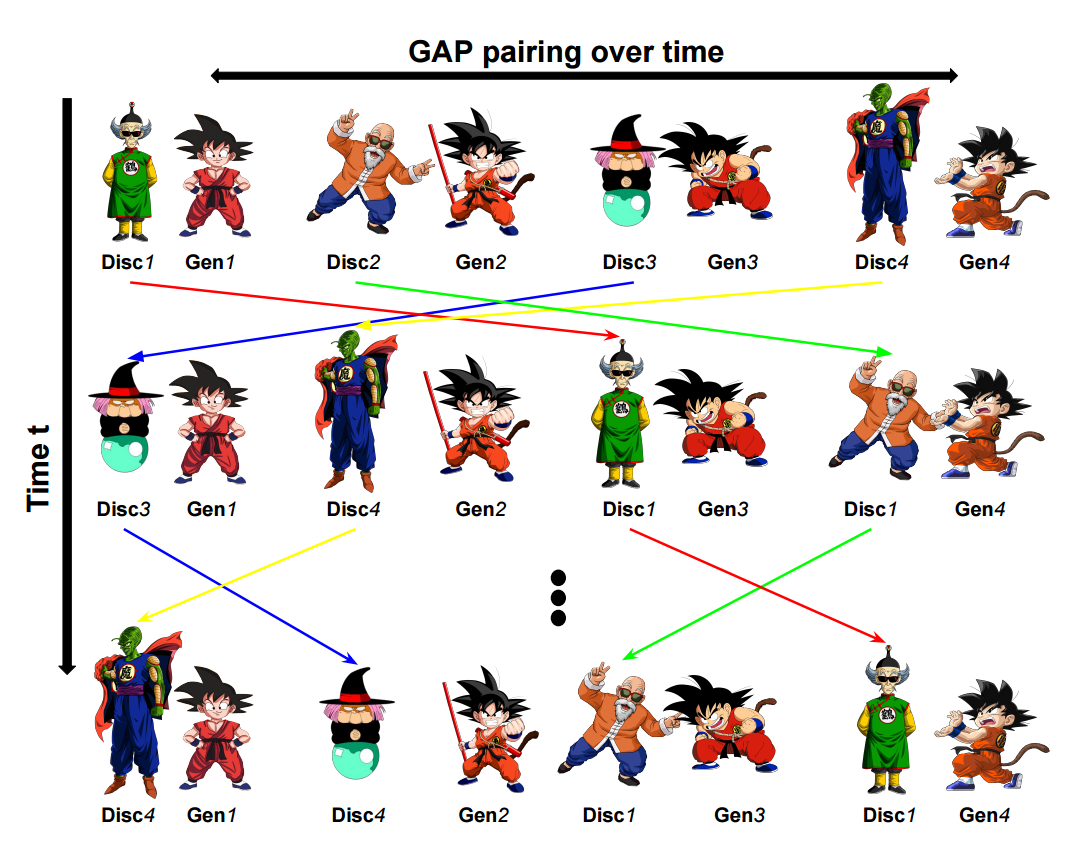
\includegraphics[scale=.3, angle=0]{Files/ParallelGAN.png}
    \caption{Cartoonization of Parallel Generative Adversarial Network}
    \label{fig:PGAN}
\end{figure}
%G. E. Hinton, S. Osindero, and Y. W. Teh. A fast learning algorithm for deep belief nets. Neural Computation,
%18(7):1527–1554, 2006